\chapter{Introduction non facultative}\label{chapIntro}

Ce chapitre présente les besoins et les concepts de la gestion de
versions d'une manière générale, ainsi qu'un aperçu des différentes
familles de systèmes de gestion de versions. Il se focalise ensuite sur
Git, qui sera l'objet du reste de cet ouvrage, pour en expliquer la
philosophie et le modèle de fonctionnement.

\section{Les besoins du génie logiciel}

La \textbf{gestion de versions}\index{gestion de versions} (en anglais
\textit{version control} ou \textit{revision control}) est une
fonctionnalité, ou plutôt une famille de fonctionnalités, qui trouve
son origine dans les besoins du développement logiciel en
équipe. Plusieurs développeurs travaillant ensemble sur le même
ensemble de fichiers, même si les domaines d'intervention de chacun
sont clairement définis, doivent nécessairement trouver un moyen de
collaborer de manière constructive, sans que les contributions des uns
ne deviennent un souci pour les autres. La gestion de version, en
s'appuyant sur un \textbf{historique}\index{historique} raisonné du
développement, a pour vocation de répondre à l'ensemble des besoins
détaillés ci-après.

\subsection{Gestion des instances du projet}

Les outils de gestion de versions doivent permettre d'identifier
plusieurs instances (éventuellement à des stades de développement
différents) du même projet. Ces instances peuvent correspondre,
suivant les cas, à l'espace de travail direct d'un développeur ou d'un
ensemble de développeurs, à une instance de référence commune partagée
par tous ou par un sous-groupe des développeurs, à une instance de
mise à disposition du public des versions stables du projet\ldots

Ces instances sont désignées sous le terme générique de
\textbf{dépôt}\index{depot@dépôt} (\textit{repository} en
anglais). Chaque dépôt est une représentation du projet. Suivant les
choix d'organisation et le système de gestion de versions utilisé, un
dépôt peut représenter le projet dans son intégralité ou bien
seulement un sous-ensemble, l'intégralité de son historique ou bien
seulement une partie. Un dépôt peut être
\textbf{local}\index{depot@dépôt!local}, c'est-à-dire situé sur la
machine de développement d'un des contributeurs (sans être
nécessairement confondu avec l'espace de travail direct du
développeur), ou bien \textbf{distant}\index{depot@dépôt!distant},
déporté sur un serveur accessible via le réseau.

\subsection{Gestion de l'historique}

La gestion de versions est un moyen de conserver une trace de
l'historique du projet (ou plus précisément d'un dépôt), sous la forme
d'un ensemble de \textbf{révisions}\index{revision@révision}
(\textit{commits} en anglais). Une révision est un ensemble atomique
et identifiable de modifications liées par une certaine unité
sémantique, portant sur un ou plusieurs fichiers, réalisées par un
même contributeur identifié, explicitement introduites dans le projet,
accompagnées d'un message explicatif et d'autres méta-données, comme
la date\footnote{Dans certains systèmes, comme par exemple
  Overleaf\index{Overleaf}, qui est une surcouche web de Git pour la
  rédaction collaborative (\url{https://www.overleaf.com/}), les
  révisions peuvent être générées automatiquement, de manière
  périodique ou à chaque modification élémentaire. Dans ce cas, une
  révision peut n'avoir ni unité sémantique ni message explicatif, ce
  qui limite forcément l'utilité de l'historique résultant. D'autre
  part, l'unicité sémantique des révisions est une propriété qui, si
  elle est désirable, dépend en grande partie de la bonne volonté des
  contributeurs\ldots}. L'atomicité signifie que les modifications
d'une même révision sont toutes appliquées ensemble au projet (ou
qu'aucune ne l'est), sans qu'une modification provenant d'une autre
révision puisse venir interférer ni que le projet puisse se retrouver
dans un état incohérent (avec une révision partiellement
appliquée)\footnote{Dans les systèmes de gestion de versions les plus
  anciens (ou les moins bien conçus), les révisions ne sont pas
  atomiques. Nous ne les mentionneront pas ici dans l'espoir que leur
  nom disparaisse à jamais de la mémoire collective et de l'histoire
  de l'informatique (pour plus de détails sur les bonnes pratiques du
  révisionnisme avec Git, les nostalgiques du Ministère de la Vérité
  \cite{Orwell} pourront étudier avec intérêt la
  section~\ref{secRevisionnisme}).}.  Par abus de langage, le terme de
révision ou de \textit{commit} désigne également l'état du projet
après application des modifications en question.

Dans le cas le plus simple, un historique est une succession linéaire
de révisions, chacune s'appuyant sur la précédente
(figure~\ref{fig:historiqueLineaire}). Dans la majorité des cas,
cependant, il en ira tout autrement\ldots\ Dans la syntaxe graphique
que nous adoptons pour les historiques, les cercles représentent les
révisions et les flèches représentent les dépendances entre
ces révisions. Le sens de ces flèches n'est donc pas le sens d'écoulement
du temps (qui va de la gauche vers la droite pour un historique
linéaire)~: le fait que la révision $E$ pointe vers la révision $D$
($D \leftarrow E$) veut dire que $E$ s'appuie sur $D$, et donc qu'elle
vient après cette dernière dans le processus de conception.

\begin{figure}[h!]
  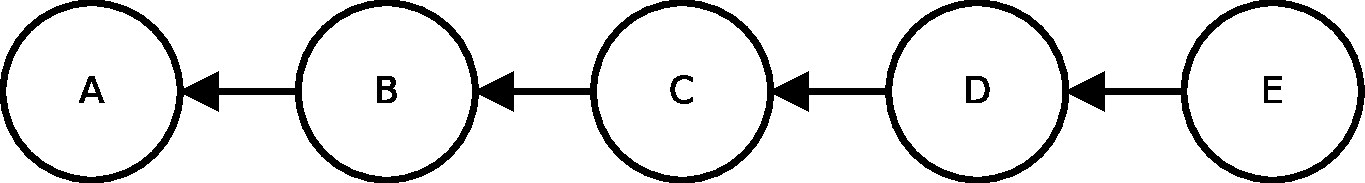
\includegraphics[width=10cm]{figures/historiqueLineaire}
  \caption{Exemple d'historique de développement linéaire, constitué
    de cinq révisions successives.\label{fig:historiqueLineaire}}
\end{figure}


L'historique a lui-même différentes utilités, au-delà de ce rôle de
représentation temporelle, notamment parce qu'il est généralement
navigable, voire cherchable. Suivant les systèmes, l'historique peut
permettre de déterminer~:
\begin{itemize}
\item La date d'introduction d'une révision donnée~;
\item L'auteur d'une révision donnée~;
\item Les modifications apportées par une révision donnée~;
\item Les causes et motivations d'une modification (si la révision
  concernée a été correctement documentée)~;
\item La révision ayant introduit une fonctionnalité, un
  bogue\index{bogue}, une régression\index{regression@régression}, une
  vulnérabilité\ldots
\item \ldots
\end{itemize}

\subsection{Intégration de contributions dans un même projet}

Les différentes personnes participant à un même projet doivent pouvoir
voir leurs contributions individuelles intégrées au projet, idéalement
de manière fluide, transparente et indolore. Le problème qui se pose
(et qui est partagé avec nombre d'autres domaines de l'informatique)
est bien évidemment celui de la concurrence entre les
modifications. Si deux développeurs, travaillant sur le même dépôt de
référence, modifient le même fichier, chacun de son côté, comment les
modifications de l'un peuvent-elles être prises en compte sans
impacter négativement (ou oblitérer complètement) le travail de
l'autre au moment d'enregistrer les révisions dans le dépôt~? Si les
deux développeurs souhaitent effectuer des modifications différentes
et jugées incompatibles par le système de gestion de versions, ce
dernier informera de l'existence d'un \textbf{conflit}\index{conflit},
qui devra être résolu avant de pouvoir continuer le développement.

La figure~\ref{fig:conflit} illustre l'apparition d'un conflit dans la
rédaction d'un document. À un certain point, le dépôt contient un
texte affirmant que les continents d'Oceania et d'Estasia sont alliés
depuis toujours dans une guerre contre Eurasia. La connaissance du
contenu de ce document est partagé de toutes les personnes ayant accès
au dépôt. Une évolution de la situation nécessite que le document soit
édité et deux rédacteurs s'attellent simultanément à la tâche, chacun
ignorant l'entreprise de l'autre. Le premier corrige le document pour
lui faire dire qu'Oceania et Eurasia sont alliés depuis toujours dans
une guerre contre Estasia, pendant que le deuxième introduit une
modification différente, reflétant sa propre vision du monde et son
expertise particulière de la
géopolitique\footnote{\url{https://en.wikipedia.org/wiki/Communications_Over_Various_Feeds_Electronically_for_Engagement_Act}.}. Ces
deux révisions traduisent des réalités complètement différentes et,
dans ce cas précis, leurs différences ne peuvent être résolues
automatiquement par un système de gestion de versions. Un conflit
survient lorsque les deux rédacteurs tentent de faire accepter leurs
révisions dans le dépôt\footnote{Le moment exact d'apparition du
  conflit et les possibiltés de résolution correspondantes dépendent
  du modèle utilisé par le système de gestion de versions.}. Un
utilisateur humain (typiquement, l'un des deux contributeurs) doit
alors intervenir pour
\textbf{résoudre}\index{conflit!resolution@résolution} le conflit et
déterminer la version du document devant apparaître dans le dépôt.

\begin{figure}[h!]
  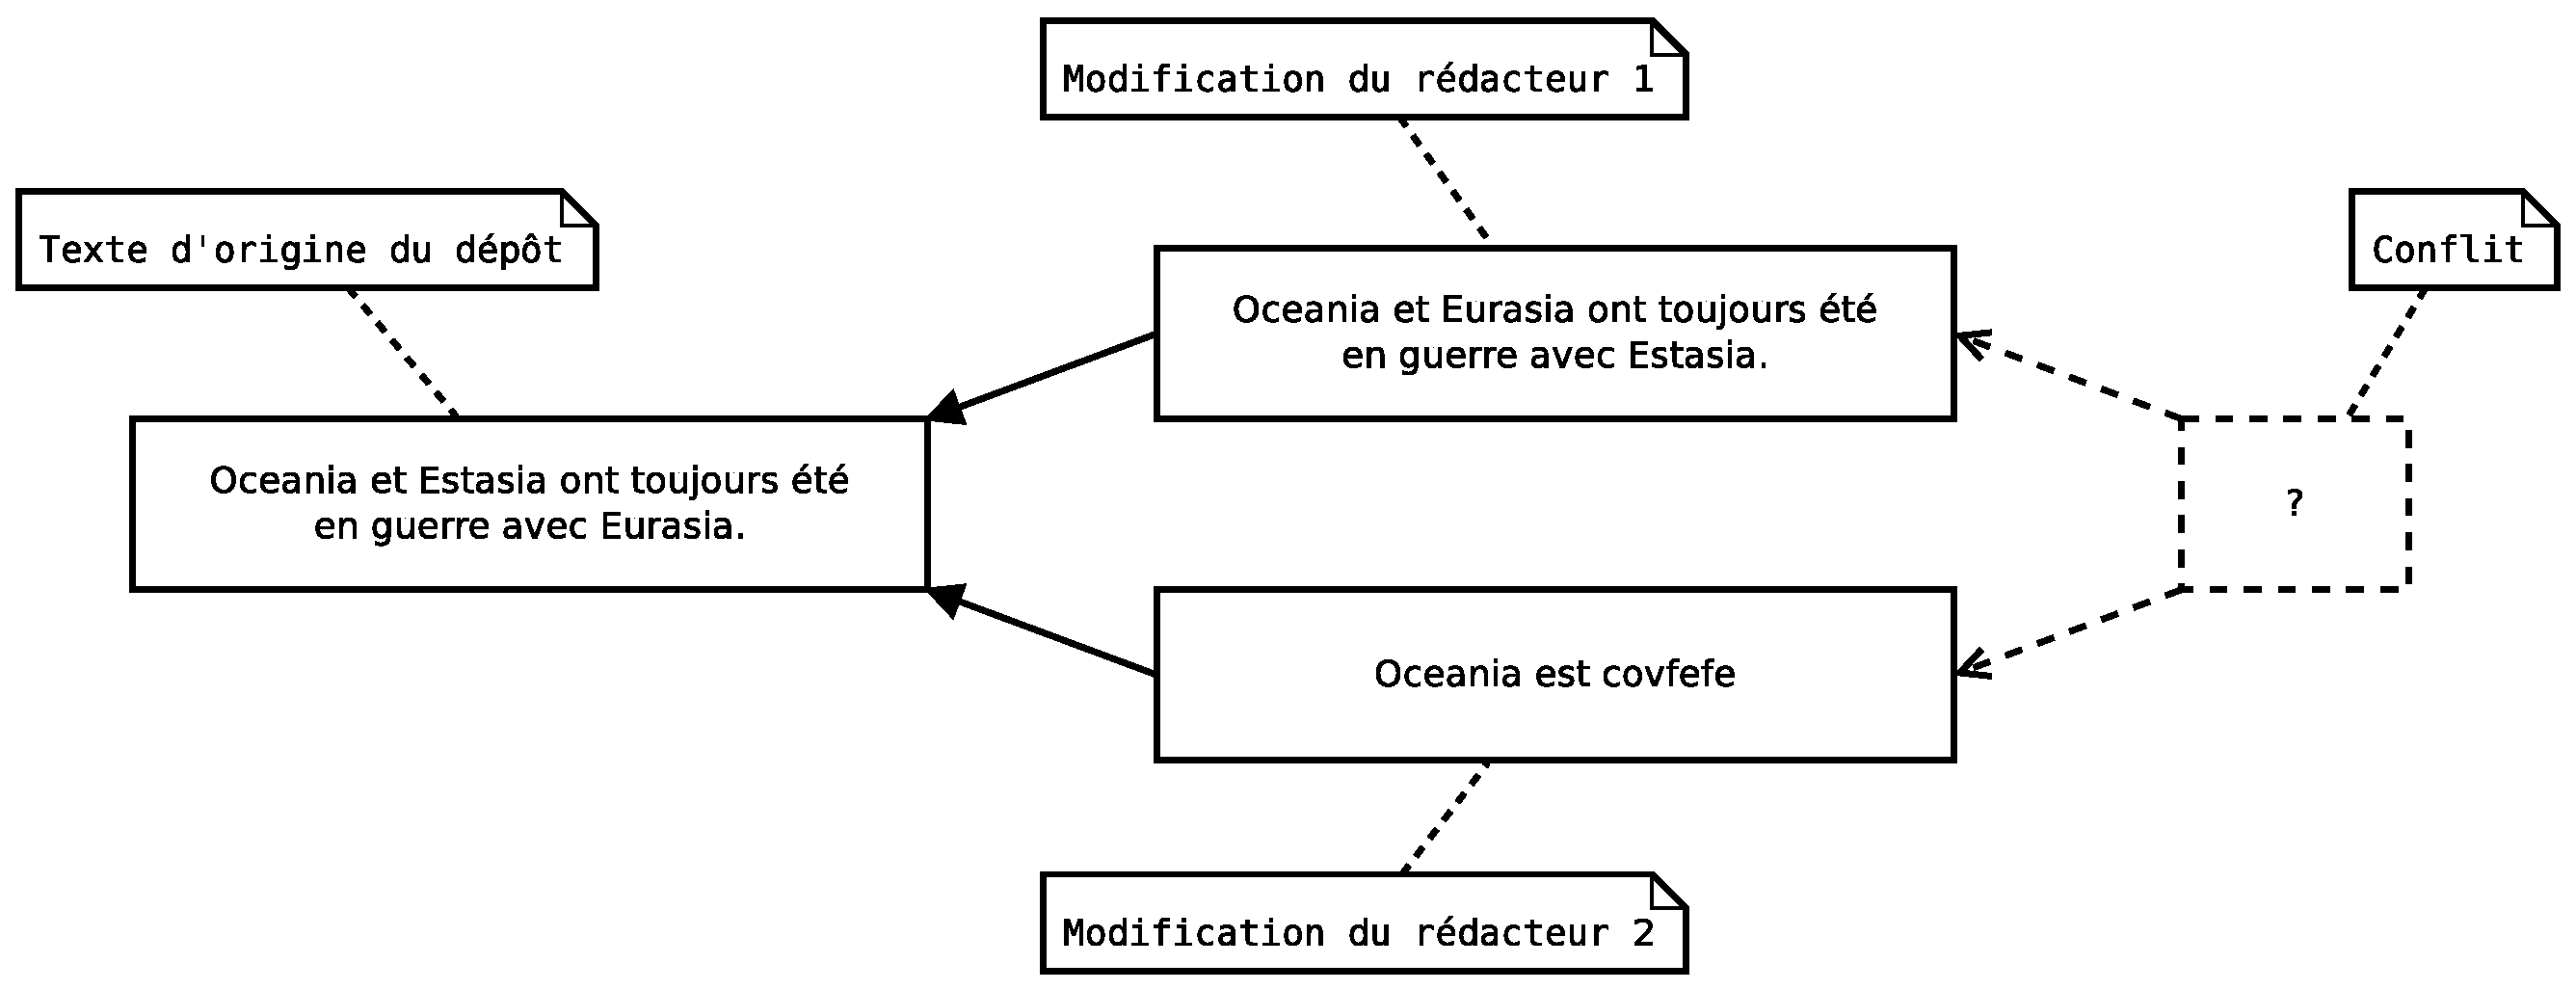
\includegraphics[width=15cm]{figures/conflit}
  \caption{Apparition d'un conflit entre les contributions de deux
    contributeurs.\label{fig:conflit}}
\end{figure}

Une première solution au problème des conflits dans les systèmes de
gestion de versions est le \textbf{verrouillage}\index{verrouillage}
des fichiers (stratégie dite \textit{lock-modify-unlock}), qui empêche
complètement l'apparition des conflits\footnote{La notion de verrou en
  informatique est utilisée dans de nombreux autres domaines dans
  lesquels se posent des problèmes de concurrence.}. Si l'on applique
cette stratégie à notre scénario, le premier rédacteur déclarera
prendre la main sur le fichier lorsqu'il commencera à travailler
dessus. Le système gérant le dépôt y posera alors un verrou. Le
deuxième rédacteur pourra toujours ouvrir le fichier en lecture, mais
aucune modification ne lui sera possible tant que le premier rédacteur
n'aura pas enregistré sa révision dans le dépôt, relâchant ainsi le
verrou. Cette stratégie de verrouillage est efficace pour éviter les
problèmes de concurrence, mais elle est très contraignante pour le
développement en équipe car elle interdit le travail simultané sur une
même portion du projet. C'est pour cela qu'elle est rarement utilisée
comme moyen principal de gestion des conflits dans les systèmes
modernes de gestion de versions\footnote{La gestion de concurrence par
  verrouillage pose en fait plusieurs types de problèmes
  \cite[chap.~1]{SVNbook}~:
  \begin{itemize}
  \item Il est possible pour un contributeur de prendre un verrou et
    de ne jamais le relâcher (parce qu'il ne valide jamais sa
    révision), nécessitant ainsi l'intervention d'un administrateur
    pour permettre aux autres développeurs de contribuer~;
  \item Des verrous inutiles peuvent être imposés, notamment lorsque
    deux contributeurs souhaitent éditer des parties différentes et
    indépendantes d'un même projet~;
  \item Le verrouillage en séquence de plusieurs fichiers par
    plusieurs contributeurs peut conduire à des interblocages~;
  \item Le verrouillage peut induire un sentiment indu de sécurité,
    alors qu'il n'empêche pas les incohérences réparties sur plusieurs
    fichiers, qui peuvent survenir si la granularité des révisions
    (dépendant généralement des usages des contributeurs) n'est pas
    adaptée.
  \end{itemize}
}.

La solution généralement retenue pour intégrer les modifications
provenant de contributeurs différents est la
\textbf{fusion}\index{fusion} (stratégie dite
\textit{copy-modify-merge}). Cette méthode consiste à toujours
accepter les modifications du premier contributeur, puis à tenter
d'accepter les modifications des suivants en essayant de les intégrer
avec les modifications déjà enregistrées. Si ces modifications n'ont
pas lieu sur les mêmes lignes de texte, la plupart des systèmes de
gestion de versions modernes pourront effectuer la fusion de manière
automatique sans lever d'alerte\footnote{Attention, le fait que des
  modifications impactent des lignes différentes ne veut pas forcément
  dire qu'elles sont compatibles, en particulier lorsqu'il s'agit de
  code source. Des modifications incohérentes entre elles à deux
  endroits du code peuvent engendrer toutes sortes d'erreurs, que le
  gestionnaire de versions ne sera pas forcément capable de
  détecter. En d'autres termes, l'absence de conflits n'est pas une
  garantie que tout s'est bien passé. D'autres outils de génie
  logiciel, comme le test systématique (intégré à des outils
  d'intégration continue comme ceux décrits dans la
  section~\ref{secCI}) ou l'analyse statique, restent nécessaires pour
  s'assurer de la qualité du code résultant.}. Dans les cas où le
système ne peut trancher lui-même, comme dans notre scénario, il
avertit le contributeur tentant d'effectuer la fusion qu'un conflit
existe, en lui présentant les différentes versions des passages posant
problème. Dans notre scénario, le deuxième rédacteur pourrait par
exemple se voir présenter le texte de la figure~\ref{fig:conflitTxt},
résultant de la fusion. Il lui reviendrait alors de déterminer la
variante du texte devant être intégrée au dépôt.

\begin{figure}[h!]
\begin{minipage}{7cm}
\begin{lstlisting}
<<<<<<< rédacteur 1
Oceania and Eurasia have always been
at war with Eastasia.
=======
Despite the constant
negative Oceania covfefe
>>>>>>> rédacteur 2
\end{lstlisting}
\end{minipage}
\caption{Exemple de conflit signalé par un gestionnaire de
  versions\label{fig:conflitTxt}}
\end{figure}

La gestion de la concurrence par fusion est une stratégie dite \og
optimiste\fg, qui table sur le fait que la majorité des fusions se
dérouleront sans problème et prévoit donc de traiter les conflits
uniquement lorsqu'ils surviennent. La gestion par verrouillage est en
revanche une stratégie dite \og pessimiste\fg, qui fait l'hypothèse
que les conflits surviennent souvent et prend donc des précautions
assez contraignantes pour les éviter. Cette dernière stratégie peut
notamment se justifier dans le traitement des fichiers non textuels
(fichers binaires, comme des exécutables ou des fichiers multimédia)
qui ne peuvent pas être fusionnés automatiquement de manière simple.

\subsection{Gestion de variantes différentes du même projet}

Un système de gestion de versions doit enfin pouvoir permettre de
créer et de maintenir simultanément des variantes distinctes du
projet, par exemple pour expérimenter l'utilisation de nouvelles
technologies, le développement de nouvelles fonctionnalités ou la mise
en place d'une nouvelle organisation. Cela est habituellement pris en
charge par le concept de \textbf{branches}\index{branche}, qui
correspond à l'idée d'un historique arborescent du développement,
plusieurs voies pouvant être suivies simultanément. La
figure~\ref{fig:historiqueArborescent} illustre un tel historique.

\begin{figure}[h!]
  \includegraphics[width=12cm]{figures/historiqueArborescent}
  \caption{Exemple d'historique de projet avec plusieurs
    branches.\label{fig:historiqueArborescent}}
\end{figure}

Cet exemple comprend trois branches identifiées~:
\begin{itemize}
\item Une branche principale (qui est appelée \texttt{trunk} dans
  Subversion et \texttt{master}\index{branches!master@\texttt{master}}
  dans Git), correspondant aux développement du projet au quotidien~;
\item Une branche de version, servant à isoler et à faire évoluer
  (notamment en lui appliquant des correctifs de sécurité) une version
  publiable du projet~;
\item Une branche correspondant au développement d'une nouvelle
  fonctionnalité. Celui-ci se fait également de manière isolée par
  rapport à la branche principale, afin de protéger cette dernière
  d'évolutions exploratoires et expérimentales (et peut-être testées
  de manière moins sévère pendant cette période de développement).
\end{itemize}
Il est à noter que dans le cas général, l'historique peut constituer
un graphe (orienté et acyclique) plutôt qu'un arbre, notamment parce
qu'il est souvent nécessaire d'intégrer les nouvelles fonctionnalités
(une fois testées et validées) dans la branche principale de
développement.

Il y a de nombreuses manières de gérer les branches d'un même projet,
notamment avec Git qui laisse le développeur très libre sur ce
point. La section~\ref{secOrgBranches} présente quelques politiques
usuelles d'organisation des différentes branches.

\section{Systèmes de gestion de version}
\index{systeme de gestion de versions@système de gestion de versions}

Ce cahier des charges du génie logiciel pour la gestion de versions
n'a pas été établi en un jour. Il est le fruit d'une longue évolution
de systèmes d'assistance au développement, répondant de plus en plus
efficacement à des besoins et des spécifications de plus en plus
riches et de plus en plus complexes. Si par la suite nous nous
focaliserons sur Git, il ne nous semble pas inintéressant de faire un
rapide état des lieux des systèmes existants (ou ayant existé). Bien
entendu, la liste proposée n'est pas exhaustive, mais elle donne un
aperçu de quelques gestionnaires de version ayant eu un certain succès
à un moment donné de l'histoire de l'informatique.

Il est globalement possible de classer ces systèmes en deux
catégories~: les systèmes \textbf{centralisés}, dans lesquels une
équipe de développement prend pour référence un dépôt unique faisant
autorité, et les systèmes \textbf{décentralisés}, permettant la
coexistence de plusieurs dépôts pour un même projet. Cette dernière
famille, arrivée plus tard dans l'historique des gestionnaires de
version, part d'un principe qui peut sembler contre-intuitif mais qui
permet pourtant une grande souplesse d'organisation et l'établissement
de procédures de collaboration très efficaces\footnote{Le modèle
  décentralisé fournit également tous les outils nécessaires à de
  véritables catastrophes logicielles et à des psychodrames très
  intéressants, s'ils sont utilisés n'importe comment.}.

S'il faut noter un point commun de la plupart des gestionnaires de
version, c'est qu'ils sont plus à l'aise dans le suivi des fichiers
textuels (typiquement les fichiers sources des langages compilables,
les scripts, les fichiers de configuration\ldots) que des fichiers
binaires (comme les documents multimédia, les exécutables, les
archives compactées\ldots). Les raisons en sont multiples. Notamment,
dans un fichier textuel il est plus facile d'identifier la portion en
conflit et de prendre automatiquement une décision de fusion qui ait
des chances d'avoir un sens. Nombre de formats binaires ne sont pas
robustes à des modifications locales~: si un gestionnaire de versions
essayait de résoudre des conflits de modifications entre deux
altérations différentes d'une même image JPEG, il y a peu de chances
que le résultat soit un document JPEG correctement formé (sans même
aller jusqu'à espérer que l'image correspondante ait quelque chose à
voir avec le résultat attendu). Les systèmes de gestion de versions
capables de traiter efficacement des formats binaires (ou des formats
textuels à la sémantique complexe) le font généralement par le biais
de greffons ou de modules d'extension spécifiques, embarquant les
informations et les analyseurs nécessaires pour interpréter et
modifier des fichiers d'un format particulier. C'est là un marché
davantage occupé par des produits propriétaires et payants.

\subsection{Systèmes centralisés} %TODO
\index{systeme de gestion de versions@système de gestion de versions!centralises@centralisé}

Les systèmes de gestion de versions centralisés font leur apparition
assez tôt dans l'histoire du développement logiciel. On peut choisir
de les catégoriser en trois générations successives \cite{Baire1}.

\subsubsection{Systèmes de première génération}

Les premiers gestionnaires de versions à être conçus présentent des
fonctionnalités bien sûr assez basiques comparés aux systèmes
actuels. Ils mettent en \oe uvre des techniques robustes et bien
connues, mais limitantes. Ils sont uniquement capable de raisonner
fichier par fichier (sans vision globale du projet, et donc sans
atomicité des révisions), d'une façon purement locale et en utilisant
des mécanismes de verrouillage pour l'évitement des conflits
d'édition.

\begin{itemize}
\item \textbf{1972~: Source Code Control System
    (SCSS)\footnote{\url{http://pubs.opengroup.org/onlinepubs/9699919799/utilities/sccs.html}.}.}\index{SCSS}
  SCSS a été développé à l'origine par Bell Labs pour des ordinateurs
  \textit{mainframe} IBM tournant sur OS/360\index{OS/360}, mais fut
  réécrit en 1977 pour tourner sur des PDP-11 sous UNIX\index{UNIX},
  système d'exploitation pour lequel il fut longtemps le gestionnaire
  de versions de référence. Il fonctionnait en introduisant des des
  fichiers source en C un identifiant textuel unique (contenant un nom
  de fichier, une date et un commentaire) qui se retrouvait ensuite
  dans les exécutables compilés, permettant d'en tracer la version des
  sources utilisée~;
\item \textbf{1982~: Revision Control System
    (RCS)\footnote{\url{https://www.gnu.org/software/rcs/}.}.}\index{RCS}
  Initialement publié comme un logiciel propriétaire, RCS est depuis
  1990 distribué sous licence GPL, et encore maintenu par le projet
  GNU. RCS utilise le concept de branches (fichier par fichier), mais
  d'une manière jugée trop complexe par les développeurs. Il introduit
  également la notion de groupes de révision (\textit{revision
    groups}), qui permet d'introduire une certaine forme d'atomicité
  transactionnelle.
\end{itemize}

\subsubsection{Systèmes de deuxième génération}

Les systèmes de gestion de versions de deuxième génération commencent
à pouvoir considérer un projet dans son ensemble, et non plus fichier
par fichier, même si l'atomicité des révisions n'est pas encore
acquise. Ils sont organisés autour d'une architecture client-serveur
et favorisent des stratégies de type \textit{merge before commit}
(c'est-à-dire que tous les conflits doivent avoir été résolus avant
d'enregistrer une révision).

\begin{itemize}
\item \textbf{1986~: Concurrent Versions System
    (CVS)\footnote{\url{http://savannah.nongnu.org/projects/cvs}.}.}\index{CVS}
  CVS, logiciel libre sous licence GPL, est la référence incontestée
  des systèmes de deuxième génération et a longtemps été le
  gestionnaire de versions le plus utilisé. Il était initialement
  conçu comme une interface d'utilisation de RCS, l'enrichissant avec
  des fonctionnalités de gestion de projet mais héritant de la
  non-atomicité de ses révisions. Le serveur CVS est normalement fait
  pour fonctionner sur UNIX\index{UNIX}, des clients existant pour les
  systèmes d'exploitation les plus courants~;
\item \textbf{1992~: Rational
    ClearCase\footnote{\url{http://www-03.ibm.com/software/products/en/clearcase}.}.}\index{Rational
    ClearCase} ClearCase a initialement été développé par Atria
  Software, maintenant intégrée à IBM. C'est un logiciel propriétaire
  (toujours maintenu) de gestion de configuration logicielle, qui
  comprend entre autres un gestionnaire de versions et qui est adapté
  à la conception conjointe du matériel et du logiciel. Il s'appuie
  sur un modèle particulier avec ses propres concepts, qui inclut
  notamment des notions de branches et de versions aux sémantiques
  prédéfinies. Il est conçu autour d'un systèmes de fichiers
  spécialisé permettant de créer des vues différentes d'un même
  projet, correspondant à des versions différentes~;
\item \textbf{1994: Microsoft Visual SourceSafe
    (VSS).}\index{Microsoft Visual SourceSafe} Visual SourceSafe est
  un logiciel propriétaire initialement développé par One Tree
  Software (depuis rachetée par Microsoft) et abandonné depuis
  2006. C'est un gestionnaire de code source (ou d'autres documents
  textuels) incluant une gestion de versions, plutôt adapté à des
  projets de petite taille. Il fait figure d'original en ceci que ses
  fonctionnalités et ses choix de conception relèvent davantage des
  systèmes de première génération. En particulier, il avait jusqu'en
  2005 la particularité de fonctionner uniquement en local
  (éventuellement sur un système de fichiers partagé) et non en mode
  client-serveur, à la différence des autres systèmes de sa
  génération. Il est également à noter qu'il fonctionnait par
  verrouillage et sans atomicité des révisions. Ces choix techniques
  ont d'ailleurs longtemps été critiqués et SourceSafe fait partie des
  rares outils de Microsoft à ne quasiment pas avoir été utilisés en
  interne. SourceSafe est maintenant remplacé, dans la suite Visual,
  par Visual Studio Application Lifecycle Management (ALM), qui peut
  interfacer d'autres gestionnaires de versions et s'appuyer sur les
  autres services fournis par Microsoft.
\end{itemize}

\subsubsection{Systèmes de troisième génération}

Les systèmes de gestion de versions centralisés les plus modernes, et
sans doute les derniers à être réellement utilisés actuellement,
assurent une véritable vision de l'historique par dépôt et par projet,
et non plus pour un simple ensemble de fichiers. L'atomicité des
révisions y est devenue un paradigme universellement partagé et
l'intégration avec différents systèmes d'exploitations et
environnements de développement une exigence assumée.

\begin{itemize}
\item \textbf{1995: Perforce
    Helix\footnote{\url{https://www.perforce.com/products/helix-core}.}.\index{Perforce
      Helix}} Originellement nommé Perforce, Perforce Helix est un
  gestionnaire de versions propriétaire développé et maintenu par la
  société du même nom. C'est un système assez répandu dans le monde
  industriel et présentant de nombreuses fonctionnalités pour
  l'utilisabilité et l'interopérabilité. La gestion des conflits
  s'appuie principalement sur la fusion mais les utilisateurs, qui
  doivent déclarer à l'avance les fichiers sur lesquels ils vont
  travailler, peuvent également choisir d'en verrouiller certains. On
  peut noter l'utilisation (encore aujourd'hui) de MD5\index{MD5} pour
  assurer l'intégrité des fichiers versionnés, ce qui fait hériter
  Perforce des vulnérabilités de cet algorithme, reconnu non sûr et
  déprécié depuis de nombreuses années~;
\item \textbf{2000: Apache Subversion
    (SVN)\footnote{\url{http://subversion.apache.org/}.}
    \cite{SVNbook}.\index{Subversion}} Subversion est le grand
  successeur de CVS pour la gestion de versions centralisée. Il a été
  initialement développé par CollabNet entre 2000 et 2004 (date de la
  première version stable) et a été accepté comme projet Apache en
  2009, avant de devenir un projet \textit{top-level} de la
  fondation. Sous licence libre depuis sa conception, il est très
  largement utilisé par la communauté libre et \textit{open source},
  tout autant que pour le développement logiciel propriétaire. Il est
  interopérable avec tous les grands systèmes d'exploitation et
  s'intègre d'une manière ou d'une autre (souvent via des greffons ou
  des modules complémentaires) dans une majorité d'environnements de
  développement. Les critiques qu'on peut lui faire (en particulier
  lorsqu'on le compare à Git) portent notamment sur ses capacités
  limitées à fusionner automatiquement des révisions concurrentes d'un
  même fichier, nécessitant des interventions manuelles fréquentes.
\end{itemize}

\subsection{Systèmes décentralisés}
\index{systeme de gestion de versions@système de gestion de versions!decentralises@décentralisé}

Les systèmes de gestion de versions décentralisés\footnote{Parfois
  qualifiés, à tort, de \og distribués\fg.} apparaissent comme une
évolution des systèmes centralisés modernes, ou comme une réaction à
ces systèmes. De la même manière, deux vagues de réflexions et de
conception ont abouti à deux générations de gestionnaires, même si
certains semblent se tenir un peu à part du fait de choix de
conception plus originaux \cite{Baire1}.

Le point commun de ces systèmes est de n'imposer ni le travail sur un
système de fichiers commun, ni une architecture client-serveur
s'appuyant sur un serveur unique. Les gestionnaires de versions
décentralisés permettent généralement de travailler avec des dépôts
multiples, dont certains peuvent par exemple être en lecture seule
(pour la publication) alors que d'autres servent au développement ou à
l'intégration. Dans ce type de systèmes, il est absolument essentiel
de disposer d'un dispositif de fusion efficace (au sens de la gestion
des conflits) et performant.

\subsubsection{Systèmes de première génération}

Les premiers gestionnaires de versions décentralisés avaient pour
principal intérêt d'être justement les premiers. La décentralisation
d'une fonctionnalité un tant soit peu complexe n'étant pas une tâche
triviale, la plupart des systèmes expérimentant ce paradigme
souffraient soit de performances dégradées, soit d'une complexité
d'utilisation rédhibitoire. Ils ont néanmoins le mérite d'avoir été
l'inspiration et le laboratoire des systèmes modernes.

\begin{itemize}
\item \textbf{2000~:
    BitKeeper\footnote{\url{http://www.bitkeeper.org/}.}.}\index{BitKeeper}
  BitKeeper est probablement l'un des premiers, sinon le premier
  gestionnaire de version décentralisé. Propriétaire, il était à
  l'origine gratuit pour les projets libres ou \textit{open
    source}. Il est notamment connu pour avoir été le système de
  gestion de versions du noyau Linux (et y avoir engendré des
  controverses animées à propos des restrictions de sa licence) entre
  2002 et 2005, date à laquelle BitKeeper a cessé d'être disponible
  gratuitement. Ce revirement, réaction à la rétro-ingénierie par un
  utilisateur du protocole de communication de BitKeeper, a constitué
  une crise et un point de rupture majeur dans l'histoire des systèmes
  de gestion de versions, incitant au développement de concurrents
  libres de très bonne qualité (Git et Mercurial). Depuis, BitKeeper
  est passé sous licence libre (Apache) mais n'a pour autant jamais
  repris sa place dans le processus de développement de Linux~;
\item \textbf{2001~: GNU
    arch\footnote{\url{https://www.gnu.org/software/gnu-arch/}.}.}\index{GNU
    arch} GNU arch est à l'origine un projet personnel de Thomas Lord,
  intégré par la suite au projet GNU. GNU arch a par la suite donné
  lieu à plusieurs dérivés (\textit{forks}), dont le plus connu est
  sans doute Baz, identifié par Thomas Lord comme son successeur
  officiel et qui a ensuite évolué en Bazaar. GNU arch a été critiqué
  pour sa difficulté de prise en main, son nombre important de
  commandes et son modèle relativement rigide~;
\item \textbf{2003~:
    Monotone\footnote{\url{http://www.monotone.ca/}.}.}\index{Monotone}
  Monotone est un gestionnaire sous licence libre (GNU GPL) qui donne
  la priorité à l'intégrité et à l'authenticité des révisions (par le
  biais de condensats SHA-1\footnote{Monotone hérite donc, comme Git
    ou Mercurial, des faiblesses de SHA-1, qui ne devrait maintenant
    plus être utilisé pour assurer l'intégrité d'un contenu, des
    collisions pouvant être construites en un temps raisonnable.} et
  de signatures RSA) par rapport aux performances. Ce choix délibéré
  se ressent particulièrement lorsqu'un nouveau contributeur doit
  cloner un dépôt pour commencer à travailler sur un projet~: de
  nombreuses vérifications cryptographiques ayant lieu à cette étape,
  le clonage peut être suffisamment long pour être réellement
  handicapant. Monotone est néanmoins réputé très robuste dans sa
  gestion des fusions et a servi d'inspiration pour le développement
  de Git.
\end{itemize}

\subsubsection{Systèmes de deuxième génération}

En 2005, au moment du mini-scandale du changement de licence de
BitKeeper, les utilisateurs des systèmes de gestion de versions
avaient accumulé suffisamment d'expérience et de frustration
collective pour exprimer de manière claire et précise les
spécifications et exigences de leur système idéal (l'abandon des
solutions centralisées étant pour beaucoup un prérequis). Il en a
résulté le développement, dans une fourchette de temps relativement
courte, de plusieurs gestionnaires de versions répondant à des
cahiers des charges similaires et relativement comparables en termes
de performance et d'utilisabilité.

\begin{itemize}
\item \textbf{2005 : GNU
    Bazaar\footnote{\url{http://bazaar.canonical.com/en/}.}.}\index{GNU
    Bazaar} Héritier indirect de GNU arch, Bazaar a été développé par
  la société Canonical, connue pour sa distribution Linux Ubuntu. Il
  était initialement pensé comme un laboratoire pour les évolutions de
  Baz mais a finalement évolué en projet autonome. Le développement a
  débuté en 2005 et la première version a été publiée en décembre
  2007. L'objectif principal de Bazaar était de reprendre les
  fonctionnalités et les principes de GNU arch, mais en revisitant
  complètement son interface de commandes, de manière à en améliorer
  l'utilisabilité. Des projets significatifs de la communauté du
  logiciel libre, comme GNU Emacs ou Bugzilla, s'appuyaient sur Bazaar
  mais l'ont abandonné au profit de Git après 2012, lorsque Canonical
  a réduit considérablement son effort de développement de Bazaar. Le
  projet est toutefois toujours officiellement maintenu~;
\item \textbf{2005 :
    Git\footnote{\url{https://git-scm.com/}.}.}\index{Git} La première
  version de Git a été développée en quelque mois par Linus Torvalds,
  après la disparition de la licence gratuite de BitKeeper pour les
  projets libres et \textit{open source}\footnote{Le nom de Git, qui
    en argot anglais désigne une personne stupide, incompétente,
    puérile ou méprisable, est à l'origine une référence de Linus
    Torvalds à lui-même, en forme d'autodérision~: \textit{``I'm an
      egotistical bastard, and I name all my projects after
      myself. First `Linux', now `git'.''} Il semblerait y avoir un
    consensus relativement large sur la prémisse de cette
    affirmation. D'autres significations et interprétations ont par la
    suite été proposées, dont la plus politiquement correcte est sans
    doute \textit{``global information tracker''}.}. Ses
  spécifications initiales sont donc ajustées aux besoins de
  développement (exigeants) du noyau Linux. Ses commandes
  raisonnablement intuitives (en tout cas, avec une certaine habitude
  des systèmes de gestion de versions), son équilibre entre
  performances et garanties d'intégrité, la souplesse d'utilisation
  commune à tous les systèmes décentralisés et surtout son adoption
  dans un projet aussi structurant en ont rapidement fait le
  gestionnaire de version distribué le plus largement adopté (et donc
  par corrolaire historique, le gestionnaire de versions le plus
  largement adopté)~;
\item \textbf{2005 :
    Mercurial\footnote{\url{https://www.mercurial-scm.org/}}.}\index{Mercurial}
  Ce gestionnaire de code source, principalement écrit en Python, a
  comme Git été motivé par le psychodrame de la licence
  BitKeeper\footnote{Le nom \og Mercurial\fg est d'ailleurs une
    critique directe de Larry McVoy, CEO de la société éditant
    BitKeeper. L'adjectif, qui lui avait été accolé dans un article,
    caractérise en anglais une personne de caractère volatil et
    changeant.}. Mercurial a été le concurrent malheureux de Git pour
  la gestion de versions du noyau Linux. L'opposition des deux
  logiciels, comparables en termes de fonctionnalités et de
  performances, reste une pomme de discorde dans la communauté du
  logiciel libre, qui s'ennuierait si elle venait à manquer de
  controverses irréductibles. Mercurial est assez couramment utilisé,
  notamment par Facebook, le W3C ou Mozilla.
\end{itemize}

\subsubsection{Autres systèmes décentralisés}

\begin{itemize}
\item \textbf{2003~: Darcs.}\index{Darcs} % TODO
\item \textbf{2006~: Fossil.}\index{Fossil} % TODO multi-fonctions (wiki, bug tracker...)
\item \textbf{2010~: Veracity.}\index{Veracity} % TODO multi-fonctions (wiki, bug tracker...)
\end{itemize}

\section{Le modèle de Git} %TODO
% TODO philosophie, différents éléments du modèle

% TODO éléments d'historique
% Développé à partir de 2005 par Linus Torvalds, pour remplacer Bitkeeper dans la gestion des sources de Git
% Juin 2005 : première release de Linux gérée avec Git
% Décembre 2005 : première release de Git

\subsection{Principes et philosophie} %TODO

% Workflow décentralisé
% Fusion facilitée
% Protection de l'intégrité (mais SHA1)...
% Performance, passage à l'échelle

\subsection{Git sur les différents systèmes d'exploitation}\label{GitOS} %TODO
\index{Windows}
\index{Linux}
\index{macOS}

\subsection{Les différents éléments du modèle} %TODO

\index{.git@\texttt{.git}}

\index{SHA1}
% TODO Expliquer en footnote que Git utilise SHA1 comme un code de
% détection d'erreur et non comme un algorithme de hachage
% cryptographique. En théorie, il est possible de falsifier le contenu
% d'un commit Git utilisant SHA1, par exemple pour y insérer du code
% malveillant, en conservant le même haché. Subversion utilise SHA1
% également, et les PDF en collision le faisaient planter, nécessitant
% un correctif. Sauf que Git utilise également SHA1 pour signer les
% commits, et là évidemment ça pose un problème d'authenticité et plus
% seulement d'intégrité.
% http://www.zdnet.fr/actualites/collision-sha-1-linus-torvalds-se-veut-rassurant-sur-git-39849070.htm
% https://twitter.com/matthew_d_green/status/835864260240683009/photo/1

\subsection{Structure d'un dépôt} %TODO
\index{depot@dépôt}
\index{depot@dépôt!local}
% TODO notion de référence

\subsection{Modèle de configuration} %TODO
\index{configuration}
\index{git@\texttt{git}!config@\texttt{config}}
\index{global@\texttt{global}}
\index{system@\texttt{system}}
\index{local@\texttt{local}}
% TODO global / system / local, principales variables